%
% File: chap01.tex
% Author: Victor F. Brena-Medina
% Description: Introduction chapter where the biology goes.
%

\let\textcircled=\pgftextcircled
\chapter{Publications composing the PhD Thesis}
\label{chap:pub}

%\initial{B}egins a chapter

%=======
\section{BEATS: Blocks of Eigenvalues Algorithm for Time Series Segmentation}
\label{sec:BEATS}

%Begins a section.


\begin{table}[ht]
\centering
\begin{tabular}{c|c}
\hline
Title & BEATS: Blocks of Eigenvalues Algorithm for Time Series Segmentation \\
\hline
\rowcolor{LightCyan}
Authors & Aurora González-Vidal, Payam Barnaghi, and Antonio F. Skarmeta \\
Type & Journal \\
\rowcolor{LightCyan}
Journal & IEEE Transactions on Knowledge and Data Engineering \\
Impact factor (2017)& 2.775 \\
\rowcolor{LightCyan}
Publisher & IEEE \\
Volume & 30  \\
\rowcolor{LightCyan}
Year & 2018 \\
ISNN& 1041-4347 (Print), 1558-2191 (Electronic) \\
\rowcolor{LightCyan}
DOI&  10.1109/TKDE.2018.2817229  \\
URL & https://ieeexplore.ieee.org/document/8319952/ \\
\rowcolor{LightCyan}
State & Published \\
Author's contribution & The author is first author... \\
\hline
\end{tabular}
\end{table}
 

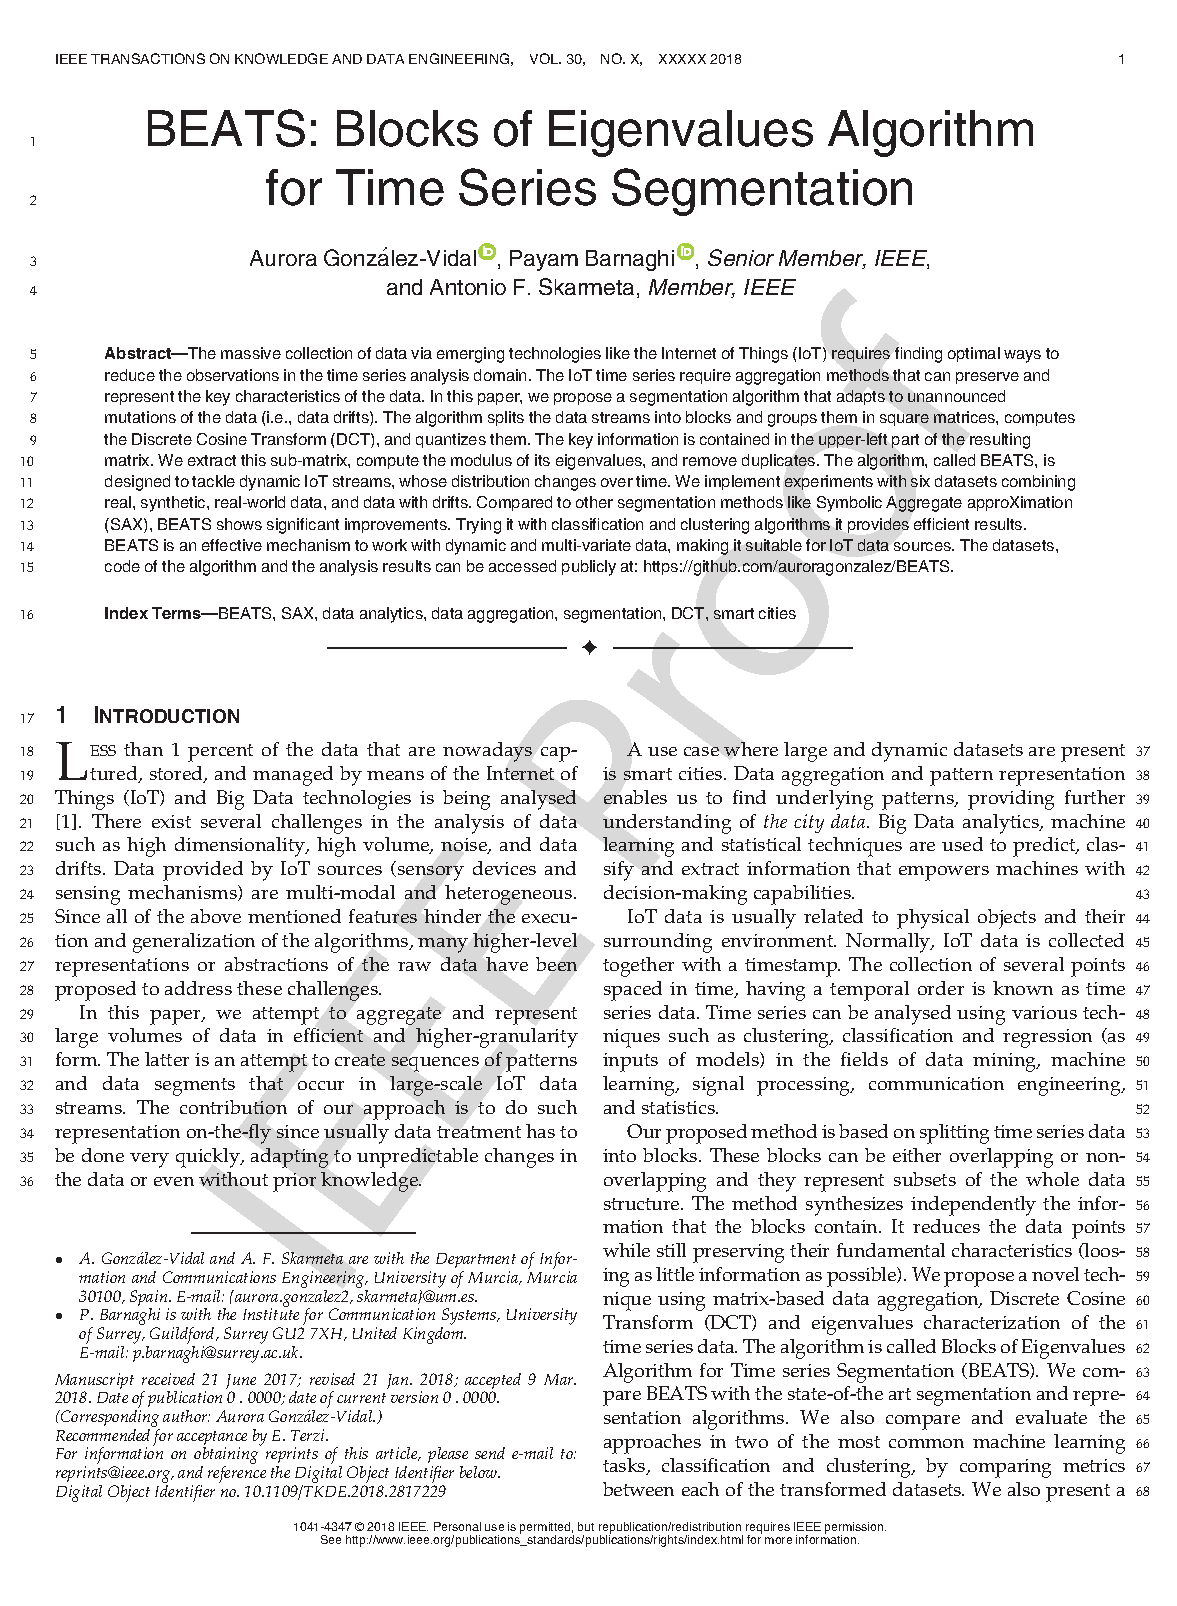
\includepdf[pages=-,pagecommand={\thispagestyle{plain}},scale=0.9]{01_BEATS2.pdf} 

\section{A methodology for Energy Multivariate Time Series Forecasting in Smart Buildings based on Feature Selection}
\label{sec:FS}

%Begins a section.




\begin{tabular}{c|c}
\hline
Title & \begin{tabular}{@{}c@{}} A methodology for Energy Multivariate Time Series Forecasting\\ in Smart Buildings based on Feature Selection \end{tabular}  \\
\hline
\rowcolor{LightCyan}
Authors & Aurora González-Vidal, Fernando Jiménez and Antonio Skarmeta-Gómez  \\
Type & Journal \\
\rowcolor{LightCyan}
Journal & Energy \\
Impact factor& \\
\rowcolor{LightCyan}
Publisher & ELSEVIER\\
Year &  \\
\rowcolor{LightCyan}
ISNN&  \\
DOI&  doi: \\
\rowcolor{LightCyan}
URL & \\
State & Published \\
\rowcolor{LightCyan}
Author's contribution &  \\
\hline
\end{tabular}
 

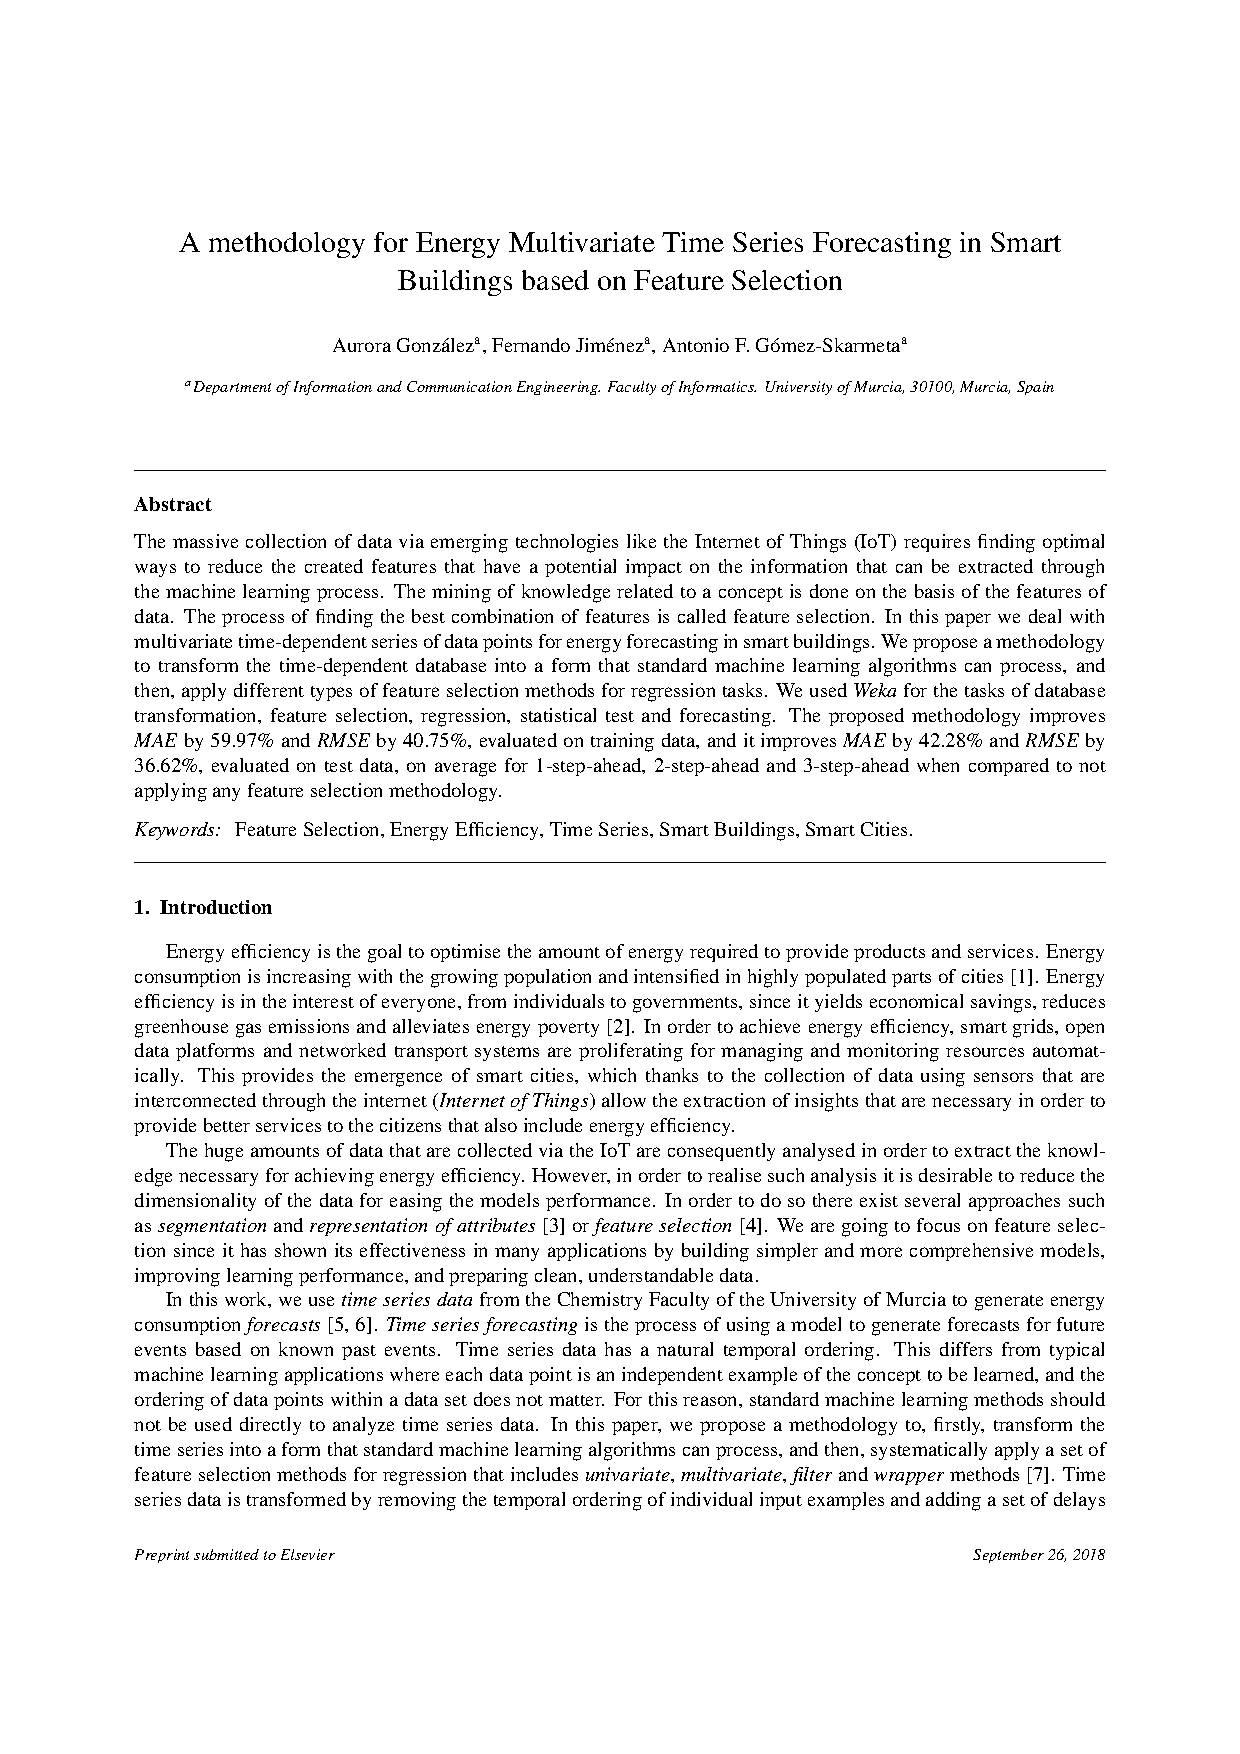
\includepdf[pages=-,pagecommand={\thispagestyle{plain}},scale=0.9]{02_FS-Energy.pdf} 





\section{Commissioning of the Controlled and Automatized Testing Facility for Human Behavior and Control (CASITA)}
\label{sec:CASITA}

%Begins a section.


\begin{tabular}{c|c}
\hline
Title &     \begin{tabular}{@{}c@{}}Commissioning of the Controlled and Automatized Testing Facility \\  for Human Behavior and Control (CASITA)\end{tabular} \\
\hline
\rowcolor{LightCyan}
Authors & 
    \begin{tabular}{@{}c@{}} Ignacio Rodríguez-Rodríguez, Aurora González-Vidal,  \\ Alfonso P. Ramallo-González and
 Miguel Ángel Zamora \end{tabular} \\
Type & Journal \\
\rowcolor{LightCyan}
Journal & Sensors \\
Impact factor (2017)& \\
\rowcolor{LightCyan}
Publisher & ELSEVIER\\
Year & 2018 \\
\rowcolor{LightCyan}
ISNN&  \\
DOI&  doi:10.3390/s18092829 \\
\rowcolor{LightCyan}
URL & \\
State & Published \\
\rowcolor{LightCyan}
Author's contribution &  \\
\hline
\end{tabular}
 

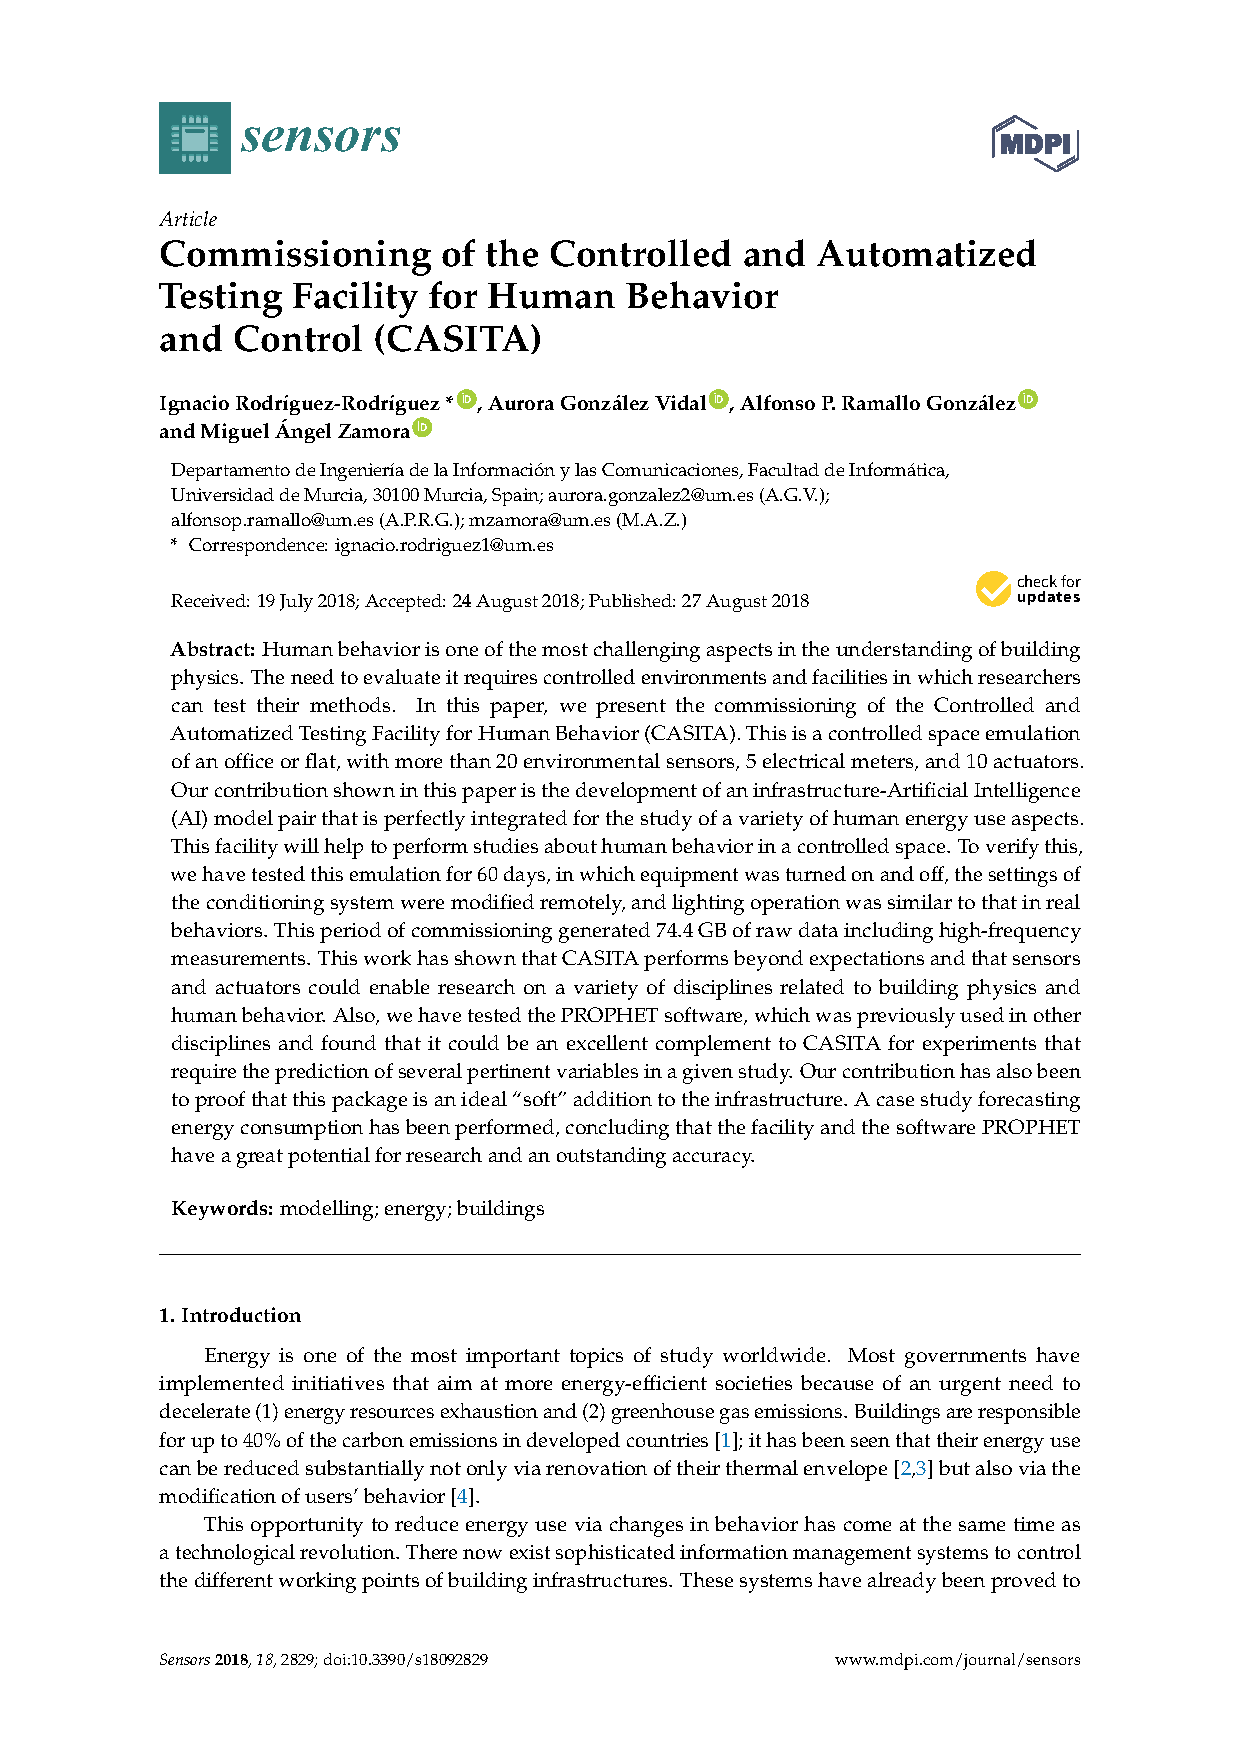
\includepdf[pages=-,pagecommand={\thispagestyle{plain}},scale=0.9]{03_CASITA.pdf} 


\section{Applicability of Big Data Techniques to Smart Cities Deployments}
\label{sec:Applica}

%Begins a section.

 
\begin{tabular}{c|c}
\hline
Title & Applicability of Big Data Techniques to Smart Cities Deployments \\
\hline
  \rowcolor{LightCyan}
   Authors & 
    \begin{tabular}{@{}c@{}c@{}}M. Victoria Moreno, Fernando Terroso-Sáenz, Aurora González-Vidal, \\ Mercedes Valdés-Vela
Antonio F. Skarmeta, Miguel A. Zamora \\ and Victor Chang\end{tabular} \\
Type & Journal \\
\rowcolor{LightCyan}
Journal & IEEE TRANSACTIONS ON INDUSTRIAL INFORMATICS \\
Impact factor (2017)& 5.43 \\
\rowcolor{LightCyan}
Publisher & IEEE \\
Volume & 13  \\
\rowcolor{LightCyan}
Issue & 2 \\
Pages &  800 - 809 \\
\rowcolor{LightCyan}
Year & 2017 \\
Month & April \\
\rowcolor{LightCyan}
ISNN& 1551-3203 (Print), 1941-0050  (Electronic) \\
DOI&  10.1109/TII.2016.2605581 \\
\rowcolor{LightCyan}
URL & https://ieeexplore.ieee.org/abstract/document/7558230/ \\
State & Published \\
\rowcolor{LightCyan}
Author's contribution & \\
\hline
\end{tabular}


\includepdf[pages=-,pagecommand={\thispagestyle{plain}},scale=0.9]{04_Applicability.pdf} 

\section{An open IoT platform for the management and analysis of energy data}
\label{sec:OpenIoT}

%Begins a section.


\begin{tabular}{c|c}
\hline
Title & An open IoT platform for the management and analysis of energy data \\
\hline
\rowcolor{LightCyan}
Authors & 
    \begin{tabular}{@{}c@{}} Fernando Terroso-Saenz, Aurora González-Vidal,  \\ Alfonso P. Ramallo-González and
Antonio F. Skarmeta \end{tabular} \\
Type & Journal \\
\rowcolor{LightCyan}
Journal & Future Generation Computer Systems \\
Impact factor (2017)& 4.639 \\
\rowcolor{LightCyan}
Publisher & ELSEVIER\\
Year & 2017 \\
\rowcolor{LightCyan}
ISNN& 0167-739X \\
DOI&  10.1016/j.future.2017.08.046 \\
\rowcolor{LightCyan}
URL & \begin{tabular}{@{}c@{}}https://www.sciencedirect.com/science/article/pii/\\ S0167739X17304181?via\%3Dihub \end{tabular} \\
State & Published \\
\rowcolor{LightCyan}
Author's contribution &  \\
\hline
\end{tabular}
 

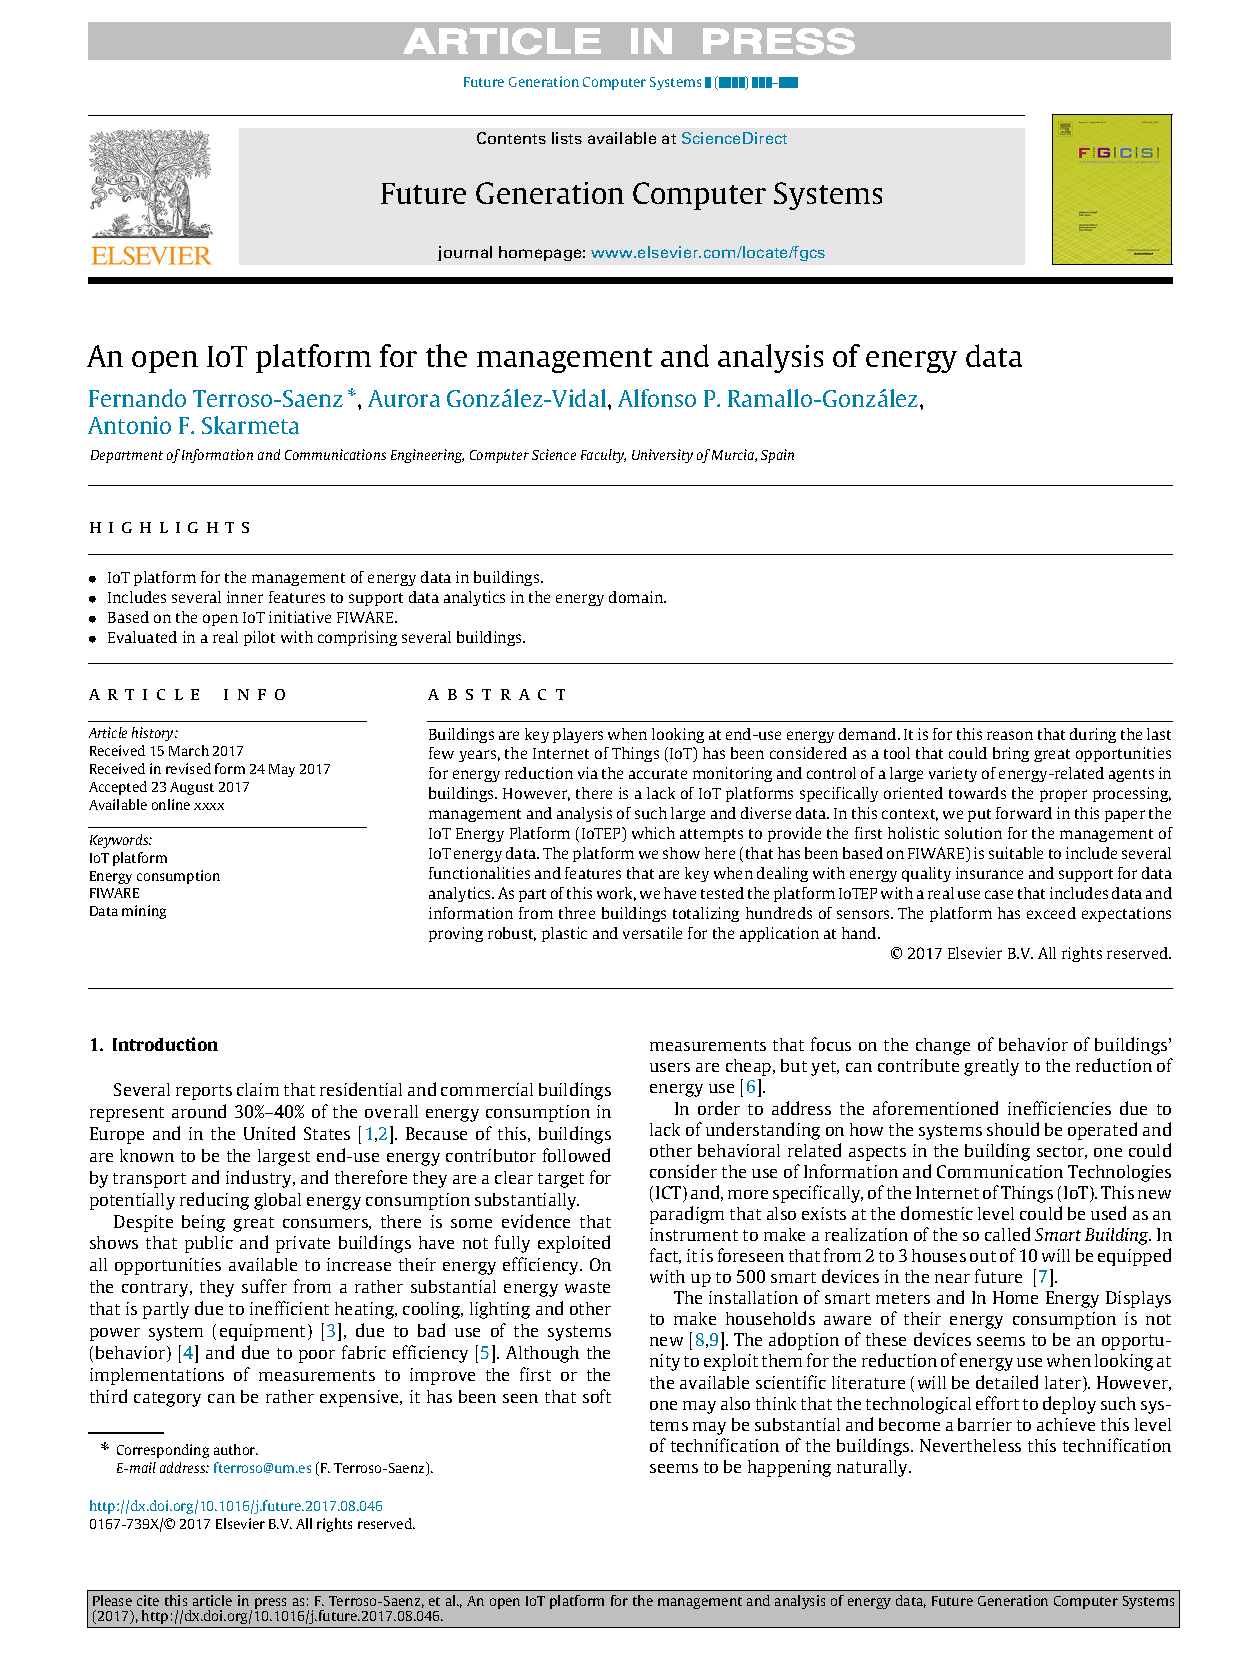
\includepdf[pages=-,pagecommand={\thispagestyle{plain}},scale=0.9]{05_AnOpenIoT.pdf} 



\section{Providing Personalized Energy Management and Awareness Services for Energy Efficiency in Smart Buildings}
\label{sec:providing}

%Begins a section.


\begin{tabular}{c|c}
\hline
Title & \begin{tabular}{@{}c@{}}Providing Personalized Energy Management and Awareness Services \\ for Energy Efficiency in Smart Buildings \end{tabular}  \\
\hline
\rowcolor{LightCyan}
Authors & 
    \begin{tabular}{@{}c@{}c@{}}Eleni Fotopoulou, Anastasios Zafeiropoulos, Fernando Terroso-Sáenz, \\ Umutcan Simsek
Aurora González-Vidal, George Tsiolis, Panagiotis Gouvas \\ Paris Liapis, Anna Fensel and Antonio Skarmeta \end{tabular} \\
Type & Journal \\
\rowcolor{LightCyan}
Journal & Sensors \\
Impact factor (2017)& 2.475 \\
\rowcolor{LightCyan}
Publisher & MDPI \\
Year & 2017 \\
\rowcolor{LightCyan}
ISNN& 1424-8220 \\
DOI&  10.3390/s17092054 \\
\rowcolor{LightCyan}
URL & https://www.ncbi.nlm.nih.gov/pubmed/28880227 \\
State & Published \\
\rowcolor{LightCyan}
Author's contribution &  \\
\hline
\end{tabular}
 

\includepdf[pages=-,pagecommand={\thispagestyle{plain}},scale=0.9]{06_Providing_personalised.pdf} 